\chapter{Tratamiento de errores}

\section{Error observacional y de modelo}

Más allá de los desafíos y dificultades de implementación de las técnicas de asimilación de datos discutidas en el capítulo anterior, la performance de estas depende crucialmente de la especificación de el error de modelo y el observacional. Tanto la evolución de las variables de estado en el tiempo como el proceso observacional tienen fuentes de incerteza. De hecho, las metodologías de asimilación de datos hacen uso de nuestro conocimiento sobre estas incertidumbres para ponderar entre la información que brinda el pronóstico producido por el modelo y la observación. Veremos que una representación incorrecta de estos errores, y en particular de la razón entre estos, puede dar lugar a un exceso de confianza en los pronósticos o en las observaciones. Esto puede ocasionar que se degrade la calidad de las estimaciones de las distribuciones filtrantes y potencialmente que el filtro se desicronice de las trayectorias subyacentes sobre las que se intenta inferir.

Las variables de estado evolucionan en el tiempo mediante la aplicación del modelo $\mathcal{M}_t$ de la ecuación \ref{eq:transition} el cual se diseña para representar la dinámica del proceso subyacente. Por supuesto, estos modelos constituyen una representación imperfecta de la realidad que buscan describir. En lo que llamamos error de modelo, no sólo incluímos este error de representatividad sino también los provenientes de aproximaciones para simplificar el cómputo, errores numéricos y posiblemente la incerteza proveniente del desconocimiento de valores exactos de la parametrización de $\mathcal{M}_t$. Llamaremos laxamente $\v Q$ al error de modelo usando la notación en \ref{eq:kf_forward} que corresponde al caso común en que lo consideremos aditivo Gaussiano e insesgado. Por otro lado, el error observacional comprende al error de representatividad del operador $\mathcal{H}_t$, las imperfecciones en su especificación y las incertezas intrínsecas de los instrumentos de medición. Análogamente al error de modelo usaremos $\v R$ para referirnos al error observacional. Tenemos entonces que $\v Q$ y $\v R$ acumulan el error de diversas fuentes de incerteza y que además en ciertos casos, como el conocimiento incompleto sobre los fenómenos que modelamos, no disponemos de una cuantificación de estas incertidumbres.

Para ilustrar la importancia de especificar correctamente $\v Q$ y $\v R$ consideremos que tenemos el modelo del oscilador armónico, totalmente observado con error de modelo $\v Q = \sigma_Q^2 \v I$ y error observacional $\v R = \sigma_R^2 \v I$. Con esta configuración generamos una trayectoria real y sus respectivas observaciones. Luego asimilamos estas observaciones con el EnKF para recuperar el estado real, pero para ello utilizaremos distintos valores de $\sigma_Q^2$ y $\sigma_R^2$. Para evaluar la performance del EnKF en cada repetición, consideraremos dos métricas: la raíz del error cuadrático medio (RMSE) y la cobertura. El RMSE nos informa cuan cerca esta la media de la estimación de la trayectoria real. Por otro lado la cobertura indica en que porcentaje la trayectoria real está incluída en las correspondientes bandas de confianza. Consideraremos un nivel de confianza del 95\% por lo que valores mayores a este indican una sobreestimación de la dispersión de la distribución filtrante mientras que valores menores corresponden a una subestimación. En la figura \ref{fig:QR_performance_trajectories} podemos ver las estimaciones del EnKF para distintas configuraciones de $\v Q$ y $\v R$ (los valores reales están indicados con $\v Q_t$ y $\v R_t$) junto con las métricas obtenidas. En el caso en que se utiliza un $\v Q < \v Q_t$ y un $\v R > \v R_t$ se tiene que la trayectoria estimada es suave, porque al subestimar el error de modelo y sobreestimar el observacional se produce el efecto de que el sistema de asimilación considera más precisos a los pronósticos que a las observaciones y por lo tanto las trayectorias prácticamente no son corregidas y se asemejan a las del modelo. Este efecto se puede ver como un subajuste (\textit{underfit}) a las observaciones y resulta en un RMSE alto; el comportamiento del filtro en esta situación en que las trayectorias prácticamente ignoran a las observaciones suele llamarse diverencia del filtro. En el caso contrario, en que $\v Q > \v Q_t$ y $\v R < \v R_t$, se tiene un efecto de sobreajuste (\textit{overfit}) a las observaciones puesto que se está subestimando su error y por lo tanto las estimaciones se acercan demasiado a ellas dando lugar a trayectorias mucho menos suaves. El caso en el que se utilicen errores de modelo y observacional menores a los reales se tiene que el RMSE es pequeño pero evidentemente la dispersión está subestimada. Por otro lado si ambos errores son mayores que los verdaderos se tiene que la dispersión está sobreestimada. El caso en que se usan los errores reales corresponde entonces a una solución de compromiso entre una correcta cobertura y un RMSE no demasiado grande. Podemos ver en los mapas de calor de la figura \ref{fig:QR_heatmap} que es importante la razón entre $\v Q$ y $\v R$: mientras este cociente es similar al cociente real entre $\v Q_t$ y $\v R_t$ se tendrá una estimación aproximadamente buena de la media, es decir bajo RMSE. Sin embargo la subestimación conjunta de ambos errores (manteniendo la razón entre ellos) produce una mala cobertura (subestimación de la dispersión) y lo contrario sucede con la sobreestimación conjunta. También se hace evidente que en la zona de \textit{overfit} (esquina inferior izquierda del panel de la derecha) se produce menos RMSE que la zona de \textit{underfit} (esquina superior derecha). Esto es debido a que cuando hay \textit{overfit} las estimaciiones tienden a interpolar las observaciones y por lo tanto se mantienen relativamente esn sincronía con las trayectorias reales pero en el caso de \textit{underfit} las estimaciones no se ven influenciadas por las obsevaciones y por lo tanto resultan también independientes de las trayectorias reales. Este análisis, desarrollado en mayor profundidad en \cite{Tandeo2020}, pone en evidencia la importancia de la estimación de estas incertezas, en particular de su especificación conjunta, para maximizar la performance de las técnicas de asimilación de datos.

\begin{figure}[h]
    \centering
    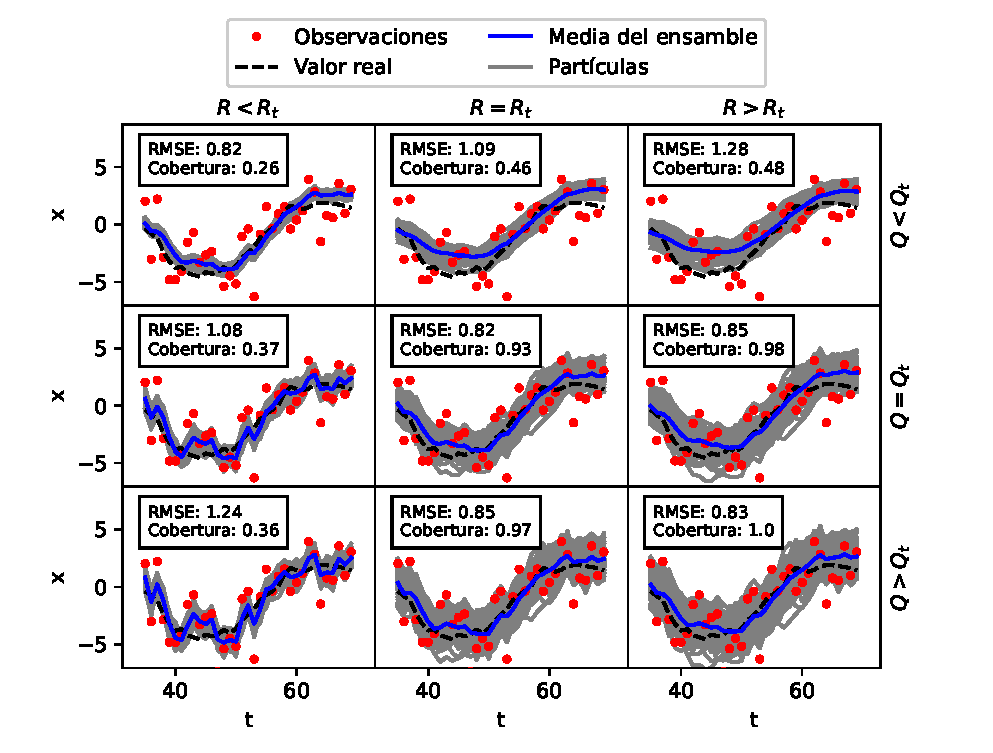
\includegraphics[width=0.75\textwidth]{QR_performance_trajectories.eps}
    \caption{Posición $x$ del oscilador armónico y estimaciones del EnKF para diferentes configuraciones de $\v Q$ y $\v R$.}
    \label{fig:QR_performance_trajectories}
\end{figure}

\begin{figure}[h]
    \centering
    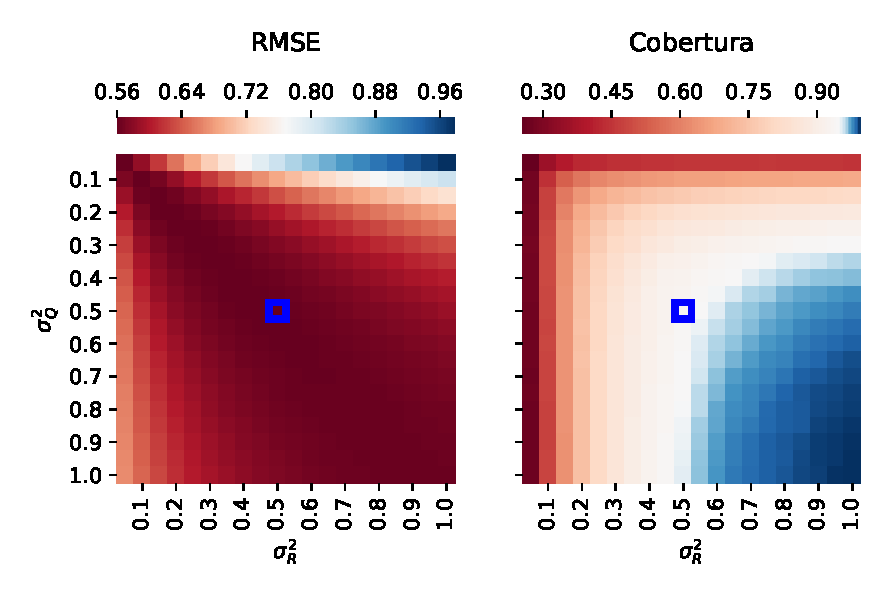
\includegraphics[width=0.75\textwidth]{QR_heatmap.eps}
    \caption{RMSE y cobertura producidas por el EnKF en la estimación del oscilador armónico para para diferentes configuraciones de $\v Q$ y $\v R$. Los valores reales se indican con un recuadro azul. La barra de colores para la cobertura tiene un escalado lineal para que el centro (color blanco) esté en el valor ópimo de cobertura de 95\%.}
    \label{fig:QR_heatmap}
\end{figure}

Como hemos visto en \ref{sec:enkf} en métodos basados en ensambles, estos tienen tendencia a colapsar debido a errores de muestreo. El error de modelo cobra una relevancia especial pues está asociada a la dispersión de las partículas del pronóstico y por lo tanto es importante especificarlo correctamente para un buen desempeño del sistema de asimilación. Por su parte, en los filtros de partículas, el error de modelo se relaciona a la incerteza de cada partícula. Muchos filtros de partículas modernos buscan mejorar el muestreo llevando a las partículas a regiones de alta verosimilitud como por ejemplo los filtros de partículas implícitos \citep{Chorin2009, Atkins2013, Zhu2016}, los filtros de flujos de partículas temperados \citep{Daum2009} o el filtro de partículas con mapeo variacional \citep{Pulido2019}. Estos suponen el conocimiento de $\v Q$ y por lo tanto se hace relevante poder acoplarlos con una metodología de estimación de dichos errores.

Se han desarrollado una gran cantidad de métodos para estimar estos errores. En \cite{Stroud2018} se apunta a maximizar la verosimilitud de las innovaciones (la diferencia entre la observación y el pronóstico mapeado al espacio observacional) utilizando inferencia Bayesiana. En otros trabajos se utilizan las covarianzas cruzadas entre innovaciones sucesivas para producir estimaciones de $\v Q$ y $\v R$ (Ver por ejemplo el trabajo seminal de \cite{Mehra1970} y una adaptación moderna basada en esta en \cite{Berry2013}). En el trabajo de \cite{Desroziers2005} se definen estadísticos de diagnóstico basados en las innovaciones que pueden ser utilizados para obtener coeficientes de inflación adaptativos \citep{Li2009}. Notemos que la inflación puede ser vista como un método de estimación del error de modelo puesto que da cuenta de la necesidad de ajustar la incertidumbre de los pronósticos. Otra aproximación al problema, sobre la que nos centraremos aquí, es la maximización de la verosimilitud total a través del algoritmo EM (\textit{expectation-maximization}, \cite{Dempster1977}). Este método fue acoplado con éxito al filtro de Kalman tradicional para estimar $\v Q$ y $\v R$ en \cite{Shumway1982} y con posteridad al filtro de Kalman por ensambles combinado con un suavizador de Kalman por ensambles (ver por ejemplo \cite{Dreano2017}). Un buen compendio de todas estas técnicas se puede encontrar en \cite{Tandeo2020}.

Dentro de toda la variedad de métodos para la estimación de errores observacionales y de modelo distinguimos los métodos \textit{offline} de los \textit{online}. Los primeros toman una ventana de observaciones $\v y_{1:T}$ y dan en base a estas una única estimación para $\v Q$ y $\v R$ para todos los tiempos $t = 1, ..., T$. El algoritmo EM es usualmente implementado de esta manera, utilizando un lote (\textit{batch}) de observaciones (tal es el caso en \cite{Dreano2017, Tandeo2015, Pulido2018}) y aplican el EnKF en combinación con el EnKS. Este procedimiento se adaptó para filtros de partículas en \cite{Lucini2021} sorteando la necesidad de utilizar un suavizador de partículas. En muchas aplicaciones no se utilizan suavizadores porque sólo hay interés en las distribuciones filtrantes y pronósticos y se implementan alternando predicción con análisis. Esto ahorra el costo computacional del suavizado y el almacentamiento de todas las estimaciones anteriores necesarias para el suavizador. En estos escenarios es impráctica o inviable la aplicación de métodos de estimación \textit{offline} y se hace necesario utilizar técnicas \textit{online} (también llamadas secuenciales o adaptativas). Estas producen estimaciones de $\v Q$ y $\v R$ de manera secuencial, es decir en cada ciclo de asimilación y utilizando la información de la observación que está siendo procesada (y no de todo el lote de observaciones de manera simultánea). En el trabajo de \cite{Neal1998} se propone una adaptación \textit{online} para el algoritmo EM y, en el contexto de modelos de Markov escondidos, podemos mencionar el algoritmo propuesto en \cite{Cappe2009} que implementa ideas de EM secuencial acoplados a filtros de partículas y las implementaciones de \cite{Andrieu2003} que utilizan pseudo-verosimilitudes basadas en mini-lotes de datos. También es necesario mencionar que existen implementaciones \textit{online} para estimación de errores que no están basadas en EM como por ejemplo la que se puede encontrar en \cite{Berry2013}.

En el trabajo del cual forma parte esta tesis, desarrollamos un nuevo método \textit{online} de estimación de error de modelo y observacional basado en EM compatible con filtros de partículas y con EnKFs. La técnica combina las ideas del \textit{batch} EM en la versón de \cite{Dreano2017} con las ideas expuestas por \cite{Cappe2009} y \cite{Andrieu2003} y el resultado está publicado en \cite{Cocucci2021}. Para dar una derivación del método desarrollaremos el algoritmo EM tradicional por lotes en \ref{sec:batchEM} y luego haremos la deducción teórica con la que podemos hacer la adaptación secuencial en \ref{sec:onlineEM}. 

\section{Estado aumentado}

En la sección anterior se dicutió la relevancia de utilizar estimaciones apropiadas de los errores involucrados. Los parámetros que codifican a estas incertezas suelen ser llamados parámetros ``estocásticos''. Por otro lado, distinguimos a los parámetros específicos al modelo transicional $\mathcal{M}_t$ los cuales suelen ser llamados parámetros ``determinísticos'' ya que usualmente son cantidades interpretables como parte de la dinámica subyacente de las variables de estado $\v x_t$. Es normal que no se cuente con un parametrización precisa del modelo de transición y por lo tanto se deban tomar recaudos. En parte, y como fue mencionado en la sección anterior, se puede dar cuenta de la imperfección en la parametrización de $\v \mathcal{M}_t$ a través del error de modelo y delegar a la estimación de este las incertezas de los parámetros determinísticos. Sin embargo, con la técnica conocida como ``estado aumentado'', es posible estimarlos individualmente y de esta manera calibrar el modelo. Esta consiste en incorporar los parámetros a las variables de estado e interpretarlas como cantidades no observadas del sistema. Si llamamos $\gv\theta_t$ a los parámetros que queremos estimar, construimos entonces el estado aumentado $\tilde{\v x}_t = (\v x_t, \gv \theta_t)$ (notemos la subindexación $t$ que incluímos porque este método admite que los parámetros varíen en el tiempo). Para poder implementar esta idea es necesario extender $\v H_t$ para que interprete a los parámetros como variables no observadas y a $\v \mathcal{M}_t$ para que actúe sobre estos.

Las técnicas de asimilación de datos pueden inferir sobre variables no observadas ya que la asimilación captura las correlaciones entre estas y las observaciones. En el caso de que esta correlación sea muy débil, el análisis será conservador respecto a la variable no observada que permanecerá cerca del pronóstico. Por lo tanto, este comportamiento se replica para los parámetros en estado aumentado y, en el caso que las correlaciones mencionadas sean los suficientemente fuertes, se podrán obtener estimaciones para los parámetros. Además, como estas estimaciones son secuenciales y siguen la lógica ``pronóstico-análisis'' como el resto de las variables de estado, es posible estimar parámetros con variación temporal dando lugar a un sistema que se auto-calibra \citep{Ruiz2013}. Sin embargo, hay que mencionar que, como los parámetros son utilizados en el modelo para el paso de tiempo subsiguiente, si los cambios en el parámetro son muy bruscos el sistema tardará en capturarlos, de manera que la adaptividad del método está sujeta a que las variaciones temporales de los parámetros sean lo suficientemente lentas como para que el sistema pueda asimilarlas. 

Para la extensión de $\v \mathcal{M}_t$ sobre los parámetros es común considerar que actúa como la identidad sobre los parámetros. Esto significa que si $\gv \theta \in \gv\Theta$ entonces $\v \mathcal{M}_t |_{\gv\Theta} (\gv \theta) = \gv \theta$. Sin embargo también habitual incorporar una caminata aleatoria Gaussiana $\v \mathcal{M}_t |_{\gv\Theta} (\gv \theta) = \gv \theta + \gv\epsilon_t$ con $\gv\epsilon_t \sim \mathcal{N}(\v 0, \gv\Sigma_{\gv\epsilon})$. Esto ayuda a que el pronóstico de los parámetros consiga una mejor exploración del espacio paramétrico. Por supuesto, se puede modelar una dinámica para la evolución de los parámetros si fuera necesario. En el caso que se utilice esta estrategia $\gv\Sigma_{\gv\epsilon}$ cuantifica la magnitud de los pasos de la caminata aleatoria y se constituye como un hiperparámetro que se puede calibrar para mejorar la performance del sistema de asimilación. 

La técnica de estado aumentado suele ser adecuada para muchos parámetros físicos y por lo tanto es tentador utilizarla para el tratamiento de los parámetros estocásticos. Sin embargo, debido a la falta de correlación entre la información observacional y los parámetros estocásticos, el método no produce buenos resultados. En \cite{Delsole2010} se puede encontrar una definición algo más precisa de parámetros determinísticos y estocásticos así como una justificación más completa de por qué aumentar el estado con parámetros estocásticos no puede dar buenas estimaciones.

\section{Algoritmo EM}

El algoritmo EM se utiliza para obtener estimadores de máxima verosimilitud en sistemas parcialmente observados. Es en realidad una metodología general y no una solución \textit{off-the-shelf}. Su aplicación más conocida es en el contexto de aprendizaje no supervisado para hacer \textit{clustering} modelando el problema con una mezcla de Gaussianas \citep{Bishop2006} pero tiene una gran diversidad de utilidades. Comenzaremos dando su forma general, luego su aplicación en lotes para estimación de matrices de covarianzas en \textit{state space models} con error aditivo Gaussiano y finalmente su adaptación \textit{online}.

El algoritmo EM en un modelo probabilístico en el que contamos con una variable observada $\v Y$, variables no observadas $\v X$ y un parámetro $\gv\theta$ el cual describe a la probbilidad conjunta $p(\v X,  \v Y; \gv\theta)$. El objetivo es utilizar datos $\v Y$ para estimar el parámetro $\gv\theta$ mediante la maximización de la verosimilitud $p(\v Y; \gv\theta)$ o equivalentemente, de su logaritmo. Si dotamos a las variables no observadas de una distribución \textit{a priori} $q(\v X)$ podemos obtener la expresión:

\begin{align}
    \log p(\v Y; \gv\theta) &=  \log \int p(\v X, \v Y; \gv\theta) d\v X \\
    &=  \underbrace{\int q(\v X) \log \frac{q(\v X)}{p(\v X | \v Y; \gv\theta)} d\v X}_{KL(\int q(\v X) \rVert p(\v X | \v Y; \gv\theta))} + \underbrace{\int q(\v X) \log \frac{p(\v X, \v Y; \gv\theta)}{q(\v X)} d\v X}_{\mathcal{L}(q, \gv\theta)} \label{eq:elbo_KL}
\end{align}
donde $KL$ es la divergencia de Kullback-Leibler y $\mathcal{L}$ es llamada ELBO (\textit{evidence lower bound}). Es común interpretar a $KL$ como una ``distancia'' entre probabilidades y de hecho, cumple que $KL(q \rVert p) \geq 0$ y se anula sí y sólo si $p = q$ en casi todo punto. Al ser $KL$ mayor o igual a 0, esto significa que $\log p(\v Y; \gv\theta) \geq \mathcal{L}(q, \gv\theta)$, es decir que la ELBO es una cota inferior de la log-verosimilitud.  

El algoritmo EM provee estimaciones $\gv\theta_0, \gv\theta_1, ...$ tales que $\log p(\v Y; \gv\theta_{t+1}) \geq \log p(\v Y; \gv\theta_t)$ que convergen a un máximo local de la verosimilitud \citep{Wu1983}. Como dado un $q$ fijo, la $\mathcal{L}(q,\gv\theta)$ es una cota inferior de $\log p(\v Y; \gv\theta)$ para todo $\gv\theta$, entonces la idea es maximizar $\mathcal{L}(q,\gv\theta)$ primero respecto a $q$ y luego respecto a $\gv\theta$. Supongamos que ya contamos con la estimación de la $t$-ésima iteración, $\gv\theta_t$. Si queremos obtener $q = \argmax\limits_{q}\mathcal{L}(q,\gv\theta_t)$, notemos que la igualdad \ref{eq:elbo_KL} se satisface para todo $q$ por lo que debemos elegir el valor que anule a la divergencia de Kullback-Leibler, es decir $q = p(\v X | \v Y; \gv\theta_t)$. Luego, dejamos fijo $q$ y elegimos $\theta_{t+1} = \argmax\limits_{\gv\theta} \mathcal{L}(q,\gv\theta)$. De esta manera obtendremos que 
\begin{align*}
    \log p(\v Y; \gv\theta_t) &= \mathcal{L}(p(\v X | \v Y; \gv\theta_t), \gv\theta_t) + \overbrace{KL(p(\v X | \v Y; \gv\theta_t) \rVert p(\v X | \v Y; \gv\theta_t))}^{0} \\
    &= \mathcal{L}(p(\v X | \v Y; \gv\theta_t), \gv\theta_t) \\
    &\leq \mathcal{L}(p(\v X | \v Y; \gv\theta_t), \gv\theta_{t+1}) \\
    % &\leq \mathcal{L}(p(\v X | \v Y; \gv\theta_t), \gv\theta_{t+1}) + \overbrace{KL(p(\v X | \v Y; \gv\theta_t) \rVert p(\v X | \v Y; \gv\theta_{t+1}))}^{\geq 0} \\
    &\leq \log p(\v Y; \gv\theta_{t+1})
\end{align*}
y por lo tanto que las estimaciones producidas incrementan la verosimilitud.

Notemos además que una vez elegido $q$ tal que anule a la divergencia de Kullback-Liebler en la iteración $t$ obtenemos que:
\begin{align*}
    \mathcal{L}(p(\v X | \v Y; \gv\theta_t), \gv\theta) &= \int p(\v X | \v Y; \gv\theta_t) \log \frac{p(\v X, \v Y; \gv\theta)}{p(\v X | \v Y; \gv\theta_t)} d\v X \\
    &= \int p(\v X | \v Y; \gv\theta_t) \log p(\v X, \v Y; \gv\theta) d\v X - \int p(\v X | \v Y; \gv\theta_t) \log p(\v X | \v Y; \gv\theta_t) d\v X \\
    &\propto_{\theta} \int p(\v X | \v Y; \gv\theta_t) \log p(\v X, \v Y; \gv\theta) d\v X \\
    &\dot{=} E_{\gv\theta_t}[\log p(\v X, \v Y; \gv\theta)| \v Y]
\end{align*}
es decir que la ELBO se puede expresar como una esperanza condicional una vez que elegimos $q$ que maximiza a $\mathcal{L}$. Debido a esto, la maximización sobre $q$ recibe el nombre de \textit{E-step}. Por otra parte el \textit{M-step} corresponde a la maximización sobre $\gv\theta$. El procedimiento admite entonces la caracterización que presentada en \ref{algo:general_EM} en el que suponemos que se realizan una cantidad prefijada $N_{it}$ de itereaciones, aunque también es posible usar otros criterios de parada.

\begin{algorithm}[H]\label{algo:general_EM}
    Elegir valor inicial $\gv\theta_0$: \\
    \For{$t=0, 1, ..., N_{it} $}{
        \textit{E-step}: \\
            \hspace{2em}Computar $\mathcal{Q}(\gv\theta, \gv\theta_t) = E_{\gv\theta_t}[\log p(\v X, \v Y; \gv\theta)| \v Y]$ \\
        
        \textit{M-step}: \\
            $\hspace{2em}\gv\theta_{t+1} = \argmax\limits_{\gv \theta} \mathcal{Q}(\gv\theta, \gv\theta_t)$
    }
\caption{EM general}
\end{algorithm}

La metodología que presentamos tiene la conveniencia de incrementar (o mantener) la verosimilitud en cada paso, sin embargo no garantiza que el máximo encontrado sea un máximo global de la verosimilitud. Por otro lado, cuando la probabilidad conjunta de las variables observadas y no observadas pertenece a la familia exponencial, tenemos simplificaciones importantes en el cómputo; esto no siempre es el caso y existen variantes del algoritmo EM que consideran hacer una maximización parcial el el \textit{M-step} (EM generalizado). Otra generalización consiste en una optimización parcial en la elección de $q$ en el \textit{E-step} (EM incremental, \cite{Neal1998}) que se implementa mediante la incorporación secuencial de las observaciones. Este método ayuda a una convergencia más rápida del algoritmo, que de otro modo tiene una convergencia en muchos casos lenta. Además, es el punto de partida para las versiones \textit{online} del EM que veremos más adelate.

\paragraph{Ejemplo EM}

Para ilustrar algunas de las características del algoritmo EM consideraremos una varible unidimendional no observada $\v X \sim \mathcal{N}(\gv\theta_t, \sigma_x^2)$ y una observación que responde al modelo $\v Y = (\v X + b)^2 + \gv \epsilon$ donde $\gv\epsilon \sim \mathcal{N}(\v 0, \sigma_y^2)$ y $b$ es un escalar. Es decir que tenemos una varible no observada que depende del parámetro verdadero $\gv\theta_t$ y una observación que corresponde a una función cuadrática de la realización de $\v X$ más ruido aditivo Gaussiano. Esto resulta en una log-verosimilitud bimodal como se representa en la figura \ref{fig:EM_example}. También se pueden ver las curvas de la ELBO para dos iteraciones del EM: se puede ver que son cotas inferiores de la log-verosimilitud y que en un punto ($\gv\theta = \gv\theta_i$) son iguales. Se puede observar en la figura que cada estimación necesariamente tendrá una verosimilitud mayor o igual al las estimaciones anteriores. Por otro lado quedan en evidencia dos de las debilidades del método: por un lado la convergencia puede ser lenta  puesto que la maximización de la ELBO puede resultar en incrementos pequeños de la verosimilitud, y por otro lado, dependiendo de la estimación inicial $\gv\theta_0$, el algoritmo puede converger a un máximo local. En este ejemplo la convergencia seríá hacia el menor de los dos máximos, pero si la estimación inicial fuera menor al valor mínimo del valle entre estos el algoritmo convergería al estimador de máxima verosimilitud. Finalmente, notemos que la difierencia entre el máximo de la ELBO para la estimación $\gv\theta_i$ y el valor de la verosimilitud en ese punto es $KL(p(\v X | \v Y; \gv\theta_{i-1}) \rVert p(\v X | \v Y; \gv\theta_{i}))$ debido a la descomposición de la verosimilitud expresada en la ecuación \ref{eq:elbo_KL}.

\begin{figure}[h]
    \centering
    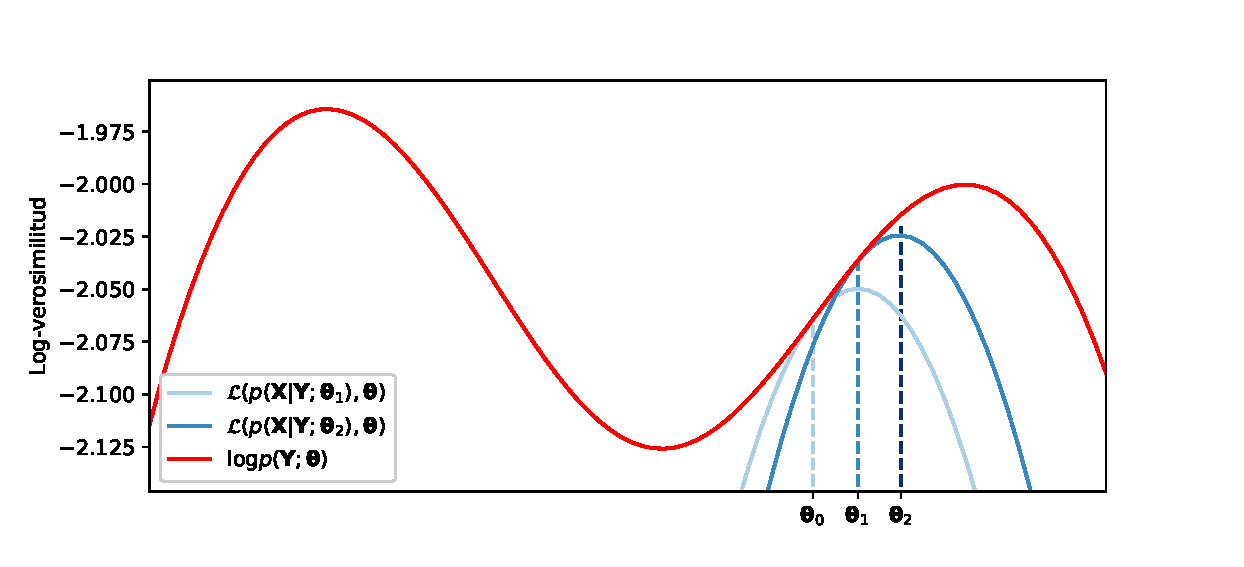
\includegraphics[width=0.75\textwidth]{EM_example.eps}
    \caption{Log-verosimilitud y ELBO para dos iteraciones del algoritmo EM}
    \label{fig:EM_example}
\end{figure}

\subsection{Batch EM} \label{sec:batchEM}

Los modelos de Markov escondidos son efectivamente sistemas parcialmente observados que en principio, admiten la aplicación del algoritmo EM. Pero además la estrctura Markoviana de dependencia temporal de las variables no observadas junto a la independencia condicional de las observaciones puede ser utilizada para obtener una expresión más sencilla de la ELBO. Haremos ahora la suposición de que contamos con un modelo de Markov escondido en un intervalo de tiempos $t = 0, 1, ..., T$ para los cuales tenemos variables latentes $\v x_{0:T}$ y observaciones $\v y_{1:T}$. Las propiedades mencionadas sobre modelos de Markov escondidos nos permiten factorizar a la probabilidad conjunta (necesaria para computar la ELBO) como:
\begin{align}
    p(\v x_{0:T}, \v y_{1:T} ; \gv\theta) &= p(\v x_0 ; \gv\theta) \prod_{t=1}^T p(\v x_t | \v x_{t-1} ; \gv\theta) p(\v y_t | \v x_t ; \gv\theta) \\
    &= p(\v x_0 ; \gv\theta) \prod_{t=1}^T p(\v x_t, \v y_t | \v x_{t-1} ; \gv\theta)
\end{align}

Con esta expresión se puede obtener entonces la siguiente para la ELBO correspondiente a la $i$-ésima iteración del método, una vez se eligió a $q$ como la distribución de las variables latentes condicionadas a las observaciones:
\begin{align}
    \mathcal{L}(p(\v x_{0:T} | \v y_{1:T} ; \gv\theta_i), \gv\theta) &\propto_{\gv\theta} \sum_{t=1}^T \int p(\v x_{1:T} | \v y_{1:T} ; \gv\theta_i) \log p(\v x_t, \v y_t | \v x_{t-1} ; \gv\theta) d\v x_{1:T} \\
    &= \sum_{t=1}^T E_{\gv\theta_i} [\log p(\v x_t, \v y_t | \v x_{t-1} ; \gv\theta) | \v y_{1:T}]
\end{align}
En esta expresión hemos quitado el término correspondiente a $p(\v x_0 ; \gv\theta)$ bajo la suposición de que no hay parametros desconocidos en la distribución inicial. Esta suposición no es necesaria y de hecho en \cite{Dreano2017} se estima su media y varianza. Ahora haremos una suposición extra que nos permitirá obtener una forma analítica del gradiente de la ELBO: supondremos que $p(\v x_t, \v y_t | \v x_{t-1} ; \gv\theta)$ pertenece a la familia exponencial. Este supuesto no es extremadamente restrictivo puesto que muchas distribuciones relevantes son de la familia exponencial incluyendo, importantemente, a la Gaussiana. Tendremos entonces que:
\begin{align*}
    p(\v x_t, \v y_t | \v x_{t-1} ; \gv\theta) = h(\v x_t, \v y_t) \exp(\psi(\gv\theta)\cdot s(\v x_{t-1}, \v x_t, \v y_t) - A(\gv\theta))
\end{align*}
donde $s(\v x_{t-1}, \v x_t, \v y_t)$ es llamado el estadístico suficiente, $\psi(\gv\theta)$ la parametrización natural y $h$ y $A$ son funciones \citep{Wasserman2004}. El gradiente de la ELBO respecto al parámetro se puede computar como:
\begin{align}
    \nabla_{\gv\theta} \mathcal{L}(p(\v x_{0:T} | \v y_{1:T} ; \gv\theta_i), \gv\theta) = \nabla_{\gv\theta} \psi(\gv\theta) \cdot \sum_{t=1}^T E_{\gv\theta_i} [s(\v x_{t-1}, \v x_t, \v y_t) | \v y_{1:T}] - T\nabla_{\gv\theta}A(\gv\theta)
\end{align}
con lo cual anulando el gradiente obtenemos la siguiente ecuación
\begin{align} \label{eq:null_elbo_grad}
    \nabla_{\gv\theta} \psi(\gv\theta) \cdot S_i - \nabla_{\gv\theta}A(\gv\theta) = 0
\end{align}
donde usamos la nomenclatura
\begin{align} \label{eq:S_def}
    S_i = \frac{1}{T}\sum_{t=1}^T E_{\gv\theta_i} [s(\v x_{t-1}, \v x_t, \v y_t) | \v y_{1:T}]
\end{align}
El valor del parámetro que cumpla con \ref{eq:null_elbo_grad} será el que maximice la ELBO y por lo tanto el valor subsiguiente del EM, $\gv\theta_{i+1}$. Más precisamente, el valor que anula el gradiente es un punto crítico pero en este caso está garantizado que es un máximo debido a propiedades del Hessiano en familias exponenciales \citep{Wainwright2008}. Notemos que la cantidad $S_i$ un promedio sobre toda la ventana temporal $t=1, .., T$ valores esperados de los estadísticos suficientes condiconados a \textit{todas} las observaciones y computado con la última estimación disponible del parámetro, $\gv\theta_i$. El condicionamiento sobre toda la ventana de observaciones implica que el valor esperado esta siendo computado utilizando las distribuciones suavizantes. El método EM que se obtiene para modelos de Markov escondidos bajo la hipótesis de familia exponencial consiste entonces en un \textit{E-step} en el que computamos $S_i$ (\ref{eq:S_def}) y un \textit{M-step} en el que resolvemos la ecuación que anula el gradiente de la ELBO (\ref{eq:null_elbo_grad}).

\subsubsection*{El caso Gaussiano}
Ahora trataremos el caso en el que el error observacional y de modelo sean aditivos y Gaussianos, es decir que tenemos:
\begin{align}
    p(\v x_t | \v x_{t-1}) &\sim \mathcal{N}(\mathcal{M}_t(\v x_{t-1}), \v Q) \\
    p(\v y_t | \v x_t) &\sim \mathcal{N}(\mathcal{H}_t(\v x_t), \v R)
\end{align}
y buscamos estimar $\gv\theta = (\v Q, \v R)$, las matrices de covarianzas del error de modelo y observacional respectivamente. Notemos que, no estamos considerando que estas matrices cambien en el tiempo, es decir que suponemos que corresponden a toda la ventana temporal. Además, debido a la independencia condicional de las observaciones de los modelos de Markov escondidos, tenemos que $p(\v x_t, \v y_t | \v x_{t-1}) = p(\v x_t | \v x_{t-1}) (\v y_t | \v x_t)$ y como supusimos que $p(\v x_t | \v x_{t-1})$ y $(\v y_t | \v x_t)$ son Gaussianas, esto implica que $p(\v x_t, \v y_t | \v x_{t-1})$ también lo es. Esto implica que seguimos bajo la suposición de familia exponencial que enunciamos anteriormente. La cantidad $S_i$, en este caso puede ser pensada como una tupla $(S_i^{\v Q}, S_i^{\v R})$ y la podemos computar mediante las siguientes expresiones que corresponden al \textit{E-step}:
\begin{align}
    S_i^{\v Q} &= \frac{1}{T}\sum_{t=1}^T E_{\gv\theta_i}[(\v x_t - \mathcal{M}_t(\v x_{t-1}))(\v x_t - \mathcal{M}_t(\v x_{t-1}))^T | \v y_{1:T}] \label{eq:batchEM_SQ} \\
    S_i^{\v R} &= \frac{1}{T}\sum_{t=1}^T E_{\gv\theta_i}[(\v y_t - \mathcal{H}_t(\v x_t))(\v y_t - \mathcal{H}_t(\v x_t))^T | \v y_{1:T}] \label{eq:batchEM_SR}
\end{align}
Por otro lado, la ecuación \ref{eq:null_elbo_grad}, para el caso Gaussiano tiene como solución exactamente a la cantidad $S_i$, con lo cual el \textit{M-step} no requiere ningún cómputo adicional. La verificación de que $\gv\theta = S_i$ anula al gradiente de la ELBO se puede encontar en el apéndice (\ref{appendix:null_grad_elbo}) junto con la representación de una densidad Gaussiana multivariada como miembro de la familia exponencial (\ref{appendix:exp_family}).

Las ecuaciones \ref{eq:batchEM_SQ} y \ref{eq:batchEM_SR}, nos dan fórmulas para computar sucesivas estimaciones de $\v Q$ y $\v R$ y constituyen las fórmulas principales utilizadas en \cite{Dreano2017, Tandeo2015, Pulido2019}. Sin embargo, requieren el cómputo de valores esperados condicionados a la totalidad de la ventana de observaciones, $\v y_{1:T}$. Si se cuenta con una representación de partículas de las distribuciones suavizantes $p(\v x_t | \v x_{1:T})$ para todo $t$, entonces los valores esperados se pueden aproximar con estimadores de Monte Carlo. Notablemente, el EnKS es una técnica que provee estas representaciones y que también es apropiada para sistemas con errores Gaussianos aditivos; por lo tanto es compatible con esta aplicación del EM. En el algoritmo \ref{algo:em_enks} podemos encontrar la implementación de este método.

\begin{algorithm}[H]\label{algo:em_enks}
    Muestrear ensamble inicial: $\{\v x_0^{a, (i)} \}_{i=1}^{N_p} \sim p(\v x_0)$ \\
    Elegir valor inicial $\gv\theta_0 = (\v Q_0, \v R_0)$:\\
    \For{$i=1, ..., N_{it}$}{
        Computar los ensambles de pronóstico, filtrantes y suavizantes usando EnKF+EnKS con la parametrización $\gv\theta_{i-1}$
            \begin{flalign*}
                \hspace{2em} \{ \v x_t^{f, (j)} \}_{j=1}^{N_p} &\sim p(\v x_t | \v y_{1:t-1}) \hspace{2em} \forall t=1, ..., T && \\
                \hspace{2em} \{ \v x_t^{a, (j)} \}_{j=1}^{N_p} &\sim p(\v x_t | \v y_{1:t}) \hspace{2em} \forall t=1, ..., T &&
            \end{flalign*}
        Utilizar los ensambles de pronóstico y filtrantes para computar los suavizantes mediante EnKS:
            \begin{flalign*}
                \hspace{2em}\{\v x_t^{s, (j)} \}_{j=1}^{N_p} \sim p(\v x_t | \v y_{1:T}) \hspace{2em} \forall t=1, ..., T &&
            \end{flalign*}
        \textit{E-step}:
            \begin{flalign*}
                \hspace{2em} S_i^{\v Q} &= \frac{1}{T} \sum_{t=1}^{T} \frac{1}{N_p} \sum_{j=1}^{N_p} (\v x_t^{s, (j)} - \mathcal{M}_t(\v x_{t-1}^{s, (j)}))(\v x_t^{s, (j)} - \mathcal{M}_t(\v x_{t-1}^{s, (j)}))^T && \\
                \hspace{2em} S_i^{\v R} &= \frac{1}{T} \sum_{t=1}^{T} \frac{1}{N_p} \sum_{j=1}^{N_p} (\v y_t - \mathcal{H}_t(\v x_t^{s, (j)}))(\v y_t - \mathcal{H}_t(\v x_t^{s, (j)}))^T &&
            \end{flalign*}
        \textit{M-step}: \\
            Asignar nuevos parámetros $\gv\theta_i = (\v Q_i, \v R_i)$
            \begin{flalign*}
                \hspace{2em} \v Q_i &= S_i^{\v Q} && \\
                \hspace{2em} \v R_i &= S_i^{\v R} &&
            \end{flalign*}
    }
\caption{EM-EnKS}
\end{algorithm}

Podemos ver que el algoritmo involucra, para cada iteración, procesar las iteraciones hacia adelante mediante predicción y filtrado con el EnKF, reprocesarlas hacia atrás con el EnKS y luego computar con Monte Carlo las actualizaciones de los parámetros. Las pasadas hacia adelante y hacia atrás provienen de que el EnKF y EnKS son implementaciones del algoritmo \textit{forward-backward}. Esto significa que para utilizar este algoritmo debemos procesar todas las observaciones reiteradas veces. Además del costo computacional, esto implica que las observaciones tienen que ser almacenadas y no se contempla una posible incorporación de nuevas observaciones, situación que sería esperable en un sistema en tiempo real. Aunque el \textit{batch EM} combinado con EnKS es un método robusto para estimar la estrctura general de $\v Q$ y $\v R$ su naturaleza \textit{offline} lo puede hacer impráctico en algunas situaciones y demasiado costoso computacionalmente. Además, no siempre es posible o factible obtener valores esperados respecto a distribuciones suavizantes. Por estos motivos se han desarrollado técnicas \textit{online} o secuenciales de estimación de parámetros estocásticos. 

\subsection{Online EM} \label{sec:onlineEM}

Aquí expondremos el algoritmo \textit{online} basado en EM cuyo desarrollo fue publicado en \cite{Cocucci2021}. El objetivo es obtener una técnica que actualice la estimación del parámetro con cada nueva observación de manera que se puedan descartar las observaciones anteriores que ya han sido procesadas. Si tomamos como punto de partida las ecuaciones \ref{eq:batchEM_SQ} y \ref{eq:batchEM_SR} podemos ver que, cada sumando corresponde a una observación pero que si quisiéramos agregar una observación nueva (correspondiente al tiempo $T+1$) todos estos sumandos deberían ser recomputados. Esto es debido a que los valores esperados están condicionados a toda la ventana observacional anterior, $\v y_{1:T}$. Las nuevas distiribuciones predictivas y filtrantes, $p(\v x_{T+1} | \v y_{1:T})$ y $p(\v x_{T+1} | \v y_{1:T+1})$ pueden ser obtenidas o aproximadas utilizando las anteriores distribuciones predictivas y filtrantes que no necesitan ser cambiadas por la incorporación de la nueva observación. Sin embargo, las distribuciones suavizantes $p(\v x_t | \v y_{1:T})$ deben ser cambiadas por las que tienen en cuenta a la nueva observación, $p(\v x_t | \v x_{1:T+1})$.

En este punto, dado que buscamos procesar observaciones que se hacen disponibles una por una, cambiaremos la notación de las iteraciones del EM y la haremos coincidir con la de las observaciones, puesto que queremos obtener una actualización de los parámetros por cada observación. Entonces consideraremos que tenemos observaciones $\v y_{1:T+1}$ y estimaciones de los parámetros $\gv\theta_0, ..., \gv\theta_T$, y buscaremos, a partir de esto, obtener la estimación $\gv\theta_{T+1}$. Más precisamente, buscaremos actualizaciones de la ELBO, es decir que dada una secuencia $S_1, ..., S_T$ buscaremos actualizar $S_T$ para que incorpore la obeservación $\v y_{T+1}$ de manera de obtener $S_{T+1}$. Esto es porque al hacer una extensión \textit{online} de el \textit{E-step} dotamos de esta propiedad a todo el algoritmo, pues el \textit{M-step} seguirá consistiendo en solucionar \ref{eq:null_elbo_grad} para $\gv\theta$ una vez computado $S_{T+1}$. Comenzamos entonces escribiendo la definición de $S_{T+1}$ como en \ref{eq:S_def} con la nueva notación y desglosando la suma de la siguiente manera:
\begin{align}
    S_{T+1} &= \frac{1}{T+1}\sum_{t=1}^{T+1} E_{\gv\theta_T} [s(\v x_{t-1}, \v x_t, \v y_t) | \v y_{1:T+1}] \\
    &= \frac{1}{T+1}\sum_{t=1}^{T+1} \int p(\v x_{t-1}, \v x_t | \v y_{1:T+1}; \gv\theta_T) s(\v x_{t-1}, \v x_t, \v y_t) d\v x_{t-1:t}\\
    &= \frac{1}{T+1} \left( \sum_{t=1}^{T} \int p(\v x_{t-1}, \v x_t | \v y_{1:T+1}; \gv\theta_T) s(\v x_{t-1}, \v x_t, \v y_t)  d\v x_{t-1:t} \right.\\ 
    &\left. + \int p(\v x_{T}, \v x_{T+1} | \v y_{1:T+1}; \gv\theta_T) s(\v x_{T}, \v x_{T+1}, \v y_{T+1}) d\v x_{T:T+1} \right)
\end{align}
Podemos identificar entonces que los primeros $T$ términos de la suma son simialres a la cantidad $TS_T$ con la salvedad de que en el condicionamiento del valor esperado se incluye la información de la última observación. Haciendo entonces la suposición de que esta última observación no afecta significativiamente a los estados anteriores y sólo influye en el último término se motiva la siguiente aproximación:
\begin{align}
    \widehat{S_{T+1}} &= \left(1 - \frac{1}{T+1}\right) \widehat{S_T} + \frac{1}{T+1} \int p(\v x_{T}, \v x_{T+1} | \v y_{1:T+1}; \gv\theta_T) s(\v x_{T}, \v x_{T+1}, \v y_{T+1}) d\v x_{T:T+1} \\
    &= (1 - \gamma_{T+1}) \widehat{S_T} + \gamma_{T+1} E_{\gv\theta_T} [s(\v x_T, \v x_{T+1}, \v y_{T+1}) | \v y_{1:T+1}] \label{eq:onlineEM_S_rescursion}
\end{align}

Tenemos entonces una fórmula que nos permite computar las aproximaciones $\widehat{S_t}$ para todo $t$ de manera recursiva en base a $S_{t-1}$. Para iniciar la recursión es necesario que contemos con una aproximación inicial $S_0$. Además introducimos $\gamma_t$ que, si bien debe valer $1/t$ para satisfacer \ref{eq:onlineEM_S_rescursion}, puede ser interpretada como una tasa de aprendizaje $\gamma_t \in (0, 1)$, tomando como inspiración técnicas de aproximación estocástica \cite{Legland1997}. Este parámetro va a controlar la ``memoria'' de los estimadores, es decir, pondera la importancia de las estimaciones anteriores respecto al nuevo térimino que incluye a la última observación. Como veremos luego este parámetro se puede calibrar para obtener comportamientos distintos del método en cuanto a convergencia. Notemos que con este esquema se puede flexibilizar la hipótesis de que los parámetros no varíán en el tiempo y podemos considerar casos en que los parámetros varíen lentamente en el tiempo. El método resultante tiene algunas similitudes con el propuesto en \cite{Cappe2009} en el que se utiliza una función auxiliar, relacionada a una forma recusiva de suavizado, que permite mantener actualizaciones de $S_t$. Podemos ver que, a pesar de evitar un suavizado hacia atrás hasta la primera observación, el cómputo del valor esperado en \ref{eq:onlineEM_S_rescursion} implica un suavizado de un paso hacia atrás porque el estadístico $s$ depende de $\v x_T$ y el condicionamiento incluye a $\v y_{T+1}$. 

En el algoritmo \ref{algo:onlineEM} se esquematiza el procedimiento de manera general. Notemos que no consideramos una ventana finita de observaciones porque potencialmente se puede seguir iterando a medida que nuevos datos se hacen disponibles. Por otro lado, no hacemos suposiciones sobre los valores iniciales pero sería natural tomar $S_0$ y $\gv\theta_0$ tales que satisfagan \ref{eq:null_elbo_grad}.

\begin{algorithm}[H]\label{algo:onlineEM}
    Elegir valor inicial para el parámetro, $\gv\theta_0$ y el estadístico, $\widehat{S_0}$: \\
    \For{$t = 1, 2, ...$}{
        \textit{E-step}: \\
        $\hspace{2em}\widehat{S_{t}} = (1 - \gamma_{t}) \widehat{S_{t-1}} + \gamma_{t} E_{\gv\theta_{t-1}} [s(\v x_{t-1}, \v x_t, \v y_t) | \v y_{1:t}] $ \\
        \textit{M-step}: \\
        Definir $\gv\theta_t$ como el valor de $\gv\theta$ que solucione: \\
        $\hspace{2em}\nabla_{\gv\theta} \psi(\gv\theta) \cdot \widehat{S_t} - \nabla_{\gv\theta}A(\gv\theta) = 0$ 
        }
        \caption{EM \textit{online}}
\end{algorithm}

De acuerdo a como se compute o aproxime el valor esperado
\begin{align}
    E_{\gv\theta_{t-1}} [s(\v x_{t-1}, \v x_t, \v y_t) | \v y_{1:t}] = \int p(\v x_{t-1}, \v x_t| \v y_{1:t} ; \gv\theta_{t-1}) s(\v x_{t-1}, \v x_t, \v y_t) d\v x_{t-1:t} \label{eq:onlineEM_expected}
\end{align}
tendremos distintas implementaciones del método. En particular daremos dos posibles formas de aproximar este valor con Monte Carlo. El primero de los métodos está basado en muestreo de importancia y está pensado para ser acoplado a filtros de partículas. La elección de la distribución de importancia evita hacer un paso de suavizado explícito. El segundo se basa en EnKF y agrega un paso hacia atrás de suavizado de manera explícita usando EnKS. 

\subsubsection*{EM \textit{online} con muestreo de importancia} \label{sec:onlineEM_IS}

Para elegir una distribución de importancia conveniente para aproximar \ref{eq:onlineEM_expected} primero desarrollaremos $p(\v x_{t-1}, \v x_t| \v y_{1:t}; \gv\theta_{t-1})$ de la siguiente manera, quitando la dependencia de $\gv\theta_{t-1}$ para mayor claridad:
\begin{align}
    p(\v x_{t-1}, \v x_t| \v y_{1:t}) &= p(\v x_t | \v x_{t-1}) p(\v x_{t-1} | \v y_{1:t-1}) \frac{p(\v y_t | \v x_t)}{p(\v y_t | \v y_{1:t-1})} \label{eq:IS_factorization}
\end{align}
En la factorización (desarrollada con mayor detalle en el apéndice \ref{appendix:IS_factorization}) podemos reconocer al modelo de transición y observacional, a la probabilidad filtrante a tiempo $t-1$ y a la cantidad $p(\v y_t | \v y_{1:t-1})$ que suele ser llamada verosimilitud marginalizada y que no depende de las variables de integración $\v x_{t-1}$ y $\v x_t$. Para aproximar entonces \ref{eq:onlineEM_expected} con muestreo de importancia debemos tener muestras de ambas variables de integración. En lugar de muestrear directamente de $p(\v x_{t-1}, \v x_t| \v y_{1:t})$ \ref{eq:IS_factorization} sugiere que podemos muestrear de $p(\v x_t | \v x_{t-1}) p(\v x_{t-1} | \v y_{1:t-1})$ y obtener pesos proporcionales a $p(\v y_t | \v x_t)$ y, mientras que nos aseguremos de normalizaizar los pesos, no debemos preocuparnos por la verosimilitud marginal. Esto es conveniente porque disponemos del modelo observacional, $p(\v y_t | \v x_t)$ para evaluar los pesos. Además, como cualquier técnica de filtrado por ensambles produce muestras de la distribución filtrante ya disponemos de las partículas correspondientes a $\v x_{t-1}$ y para obtener las de $\v x_t$ podemos utilizar el modelo de transición.

Si estamos utilizando un método por ensambles de $N_p$ partículas, podemos utilizar nuestra muestra de la ditribución filtrante,
\begin{align*}
    \{ \v x_{t-1}^{a, (j)}\}_{j=1}^{N_p} \sim p(\v x_{t-1} | \v y_{1:t-1} ; \gv\theta_{t-1})
\end{align*}
y en base a cada partícula de esta muestra obtener otra, cuyo tamaño denominamos $M_p$, correspondiente a $\v x_t$:
\begin{align*}
    \{ \v x_{t}^{f, (j,l)}\}_{l=1}^{M_p} \sim p(\v x_t | \v x_{t-1}^{a, (j)} ; \gv\theta_{t-1})
\end{align*}
Estas últimas $N_p M_p$ partículas llevan el superíndice $f$ pues se obtienen de la misma manera en que se obtendría un pronóstico (\textit{forecast}) pero haciendo la salvedad de que tenemos $M_p$ partículas por cada punto del tiempo anterior. Con estas muestras podemos ya calcular los pesos no normalizados,
\begin{align*}
    \overline{w_{j,l}} = p(\v y_t | \v x_t^{(j,l)})
\end{align*}
y una vez que obtenemos las versiones normalizadas, $w_{j,l}$ podemos hacer la aproximación de Monte Carlo de la integral:
\begin{align*}
    E_{\gv\theta_{t-1}} [s(\v x_{t-1}, \v x_t, \v y_t) | \v y_{1:t}] \approx \sum_{j=1}^{N_p} \sum_{l=1}^{M_p} w_{j, l} s(\v x_{t-1}^{a, (j)}, \v x_{t}^{f, (j,l)}, \v y_t)
\end{align*}

Este método puede ser implementado con cualquier técnica de asimilación de datos por ensambles ya que solo necesitamos: una representación de partículas filtrante, evaluar el modelo observacional ($p(\v y_t | \v x_t)$) y muestrear del modelo de transición ($p(\v x_t | \v x_{t-1})$), es decir evolucionar el modelo hacia adelante. Por lo tanto, la metodología es compatible con EnKF y filtros de partículas. Notemos también que  es posible tomar $M_p = 1$ pues esto es equivalente a muestrear $(\v x_{t-1}, \v x_t)$ de manera conjunta de la distribución $p(\v x_t | \v x_{t-1}) p(\v x_{t-1} | \v y_{1:t-1}) = p(\v x_t, \v x_{t-1} | \v y_{1:t-1})$. El algoritmo \ref{algo:onlineEM_IS} especifica el método.

\begin{algorithm}[H]\label{algo:onlineEM_IS}

    Muestrear partículas iniciales: $\{\v x_0^{(j)}\}_{j=1}^{N_p} \sim p(\v x_0)$ \\
    Elegir valor inicial para el parámetro, $\gv\theta_0$ y el estadístico, $\widehat{S_0}$: \\
    \For{$t = 1, 2, ...$}{
    Calcular pesos:\\
    \For{$j=1, ..., N_p$}{
        \For{$l=1, ..., M_p$}{
                $\v x_{t}^{f, (j,l)} \sim p(\v x_{t} | \v x_{t-1}^{a, (j)};\gv\theta_{t-1})$ \\
                $w_{j,l} \propto p(\v y_{t} | \v x_{t}^{f, (j,l)} ; \gv\theta_{t-1})$
        }
    }
    Muestrear partículas filtrantes:\\
    $\hspace{2em}\{\v x_{t}^{a, (j)}\}_{j=1}^{N_p}  \sim p(\v x_{t} | \v y_{1:t};\gv\theta_{t-1})$\\
    Computar $\widehat{S_t}$: \\
    $\hspace{2em}\widehat{S_{t}} = (1 - \gamma_{t}) \widehat{S_{t-1}} + \gamma_{t} \sum_{j=1}^{N_p} \sum_{l=1}^{M_p} w_{j, l} s(\v x_{t-1}^{a, (j)}, \v x_{t}^{f, (j,l)}, \v y_t) $ \\
    Definir $\gv\theta_t$ como el valor de $\gv\theta$ que solucione: \\
    $\hspace{2em}\nabla_{\gv\theta} \psi(\gv\theta) \cdot \widehat{S_t} - \nabla_{\gv\theta}A(\gv\theta) = 0$
    }
\caption{EM \textit{online} con muestreo de importancia}
\end{algorithm}

\subsubsection*{EM \textit{online} con un paso de suavizado} \label{sec:onlineEM_OSS}

Otra alternativa para obtener una aproximación de Monte Carlo de \ref{eq:onlineEM_expected} es muestrear directamente de $p(\v x_{t-1}, \v x_t| \v y_{1:t})$ para lo cual es necesario obtener la versión suavizada del estado a tiempo $t-1$. El EnKF puede proveernos las partículas correspondientes a $p(\v x_t | \v y_{t-1})$ mientras que podemos obtener una muestra de $p(\v x_{t-1} | \v y_{1:t})$ mediante el EnKS, presentado en el algoritmo \ref{algo:enks}. Notemos además que no es necesario iterar con el EnKS hasta la primera observación sino que basta con hacer un solo paso hacia atrás pues sólo no estamos interesados en las partículas que coresponden a tiempos anteriores a $t-1$. De esta manera, muestreamos:
\begin{align*}
    \{\v x_t^{a, (j)}\}_{j=1}^{N_p} &\sim p(\v x_t | \v x_{1:t}) \\
    \{\v x_t^{s, (j)}\}_{j=1}^{N_p} &\sim p(\v x_{t-1} | \v x_{1:t})
\end{align*}
donde las partículas suavizantes pueden ser obtenidas del ensamble de pronóstico y el filtrante utilizando las siguientes expresiones:
\begin{align*}
    \v K_{t-1}^s &= \v S_{t-1}^a ( {\v S_t^f}^T \v S_t^f )^{-1} {\v S_t^f}^T \\
    \v x_{t-1}^{j, (s)} &= \v x_{t-1}^{j, (s)} + \v K_{t-1}^s (\v x_t^{j, (s)} - \v x_t^{j, (f)})
\end{align*}
Notemos que, cuando $\v y_t$ es la última observación disponible, la distribución filtrante coincide con la suavizante a ese tiempo y por lo tanto $\v x_t^{s, (j)} = \v x_t^{a, (j)}$. La aproximación de Monte Carlo resulta entonces en:
\begin{align*}
    E_{\gv\theta_{t-1}} [s(\v x_{t-1}, \v x_t, \v y_t) | \v y_{1:t}] \approx \sum_{j=1}^{N_p} s(\v x_{t-1}^{s, (j)}, \v x_{t}^{a, (j)}, \v y_t)
\end{align*}
y la meteodología puede ser entonces expresada en forma algorítmica como se expone en \ref{algo:onlineEM_OSS}.

\begin{algorithm}[H]\label{algo:onlineEM_OSS}
    
    Muestrear partículas iniciales: $\{\v x_0^{(j)}\}_{j=1}^{N_p} \sim p(\v x_0)$ \\
    Elegir valor inicial para el parámetro, $\gv\theta_0$ y el estadístico, $\widehat{S_0}$: \\
    \For{$t = 1, 2, ...$}{
        Computar partículas filtrantes y suavizantes utilizando EnKF+EnKS:\\
    $\hspace{2em}\{\v x_t^{a, (j)}\}_{j=1}^{N_p} \sim p(\v x_t | \v y_{1:t};\gv\theta_{t-1})$ \\
    $\hspace{2em}\{\v x_{t-1}^{s, (j)}\}_{j=1}^{N_p} \sim p(\v x_{t-1} | \v y_{1:t};\gv\theta_{t-1})$ \\
    Computar $\widehat{S_t}$: \\
    $\hspace{2em}\widehat{S_{t}} = (1 - \gamma_{t}) \widehat{S_{t-1}} + \gamma_{t} \frac{1}{N_p}\sum_{j=1}^{N_p} s(\v x_{t-1}^{s, (j)}, \v x_{t}^{a, (j)}, \v y_t) $ \\
    Definir $\gv\theta_t$ como el valor de $\gv\theta$ que solucione: \\
    $\hspace{2em}\nabla_{\gv\theta} \psi(\gv\theta) \cdot \widehat{S_t} - \nabla_{\gv\theta}A(\gv\theta) = 0$
    }
    \caption{EM \textit{online} con suavizado de un paso}
\end{algorithm}
No especificamos que implementación de EnKF o EnKS utilizamos porque potencialmente podemos elegir la que resulte más conveniente. Al estar basado en el filtro de Kalman por ensambles, valen los requerimientos usuales para dicho método, es decir errores aditivos Gaussianos en el modelo de transición y observacional. Si consideramos que en el caso Gaussiano, el estadístico suficiente 
se puede expresar como $s(\v x_{t-1}, \v x_t, \v y_{1:t}) = (s^Q(\v x_{t-1}, \v x_t), s^R(\v y_t, \v x_t))$ donde
\begin{align*}
    s^Q(\v x_{t-1}, \v x_t) &= (\v x_t - \mathcal{M}_t(\v x_{t-1}))(\v x_t - \mathcal{M}_t(\v x_{t-1}))^T \\
    s^R(\v y_t, \v x_t) &= (\v y_t - \mathcal{Y}_t(\v x_t))(\v y_t - \mathcal{H}_t(\v x_t))^T
\end{align*}
podemos ver la similaridad entre este método y el EM-EnKS presentado en el algoritmo \ref{algo:em_enks}. Sin embargo, si aplicaramos  la versión \textit{online} a una ventana de tiempo $t = 1, ..., T$, podemos ver que este realiza aproximadamente la misma cantidad de operaciones en total que una única iteración de la versión \textit{offline}. De hecho, el EM \textit{online} requerirá $T$ pasos temporales de EnKF y $T$ pasos simples (de una sola observación) hacia atrás de EnKS: esto es equivalente al pase completo de EnKF+EnKS en la versión \textit{batch}. Por otro lado, la cantidad de evaluaciones de $s$ en el pase completo de la versión \textit{online} es $N_pT$, lo cual coincide con una única iteración del \textit{offline}.
